\documentclass[a4paper, 12pt, final, garamond]{book}
\usepackage{cours-preambule}

\raggedbottom

\makeatletter
\renewcommand{\@chapapp}{M\'ecanique -- chapitre}
\makeatother

\begin{document}
\setcounter{chapter}{4}

\chapter{Correction TD application}

\section{Mouvements simples de particules chargées}
\begin{enumerate}
    \item On étudie la particule M de masse $m$ et de charge $q$ assimilée à
        un point matériel dans le référentiel du laboratoire supposé galiléen.
        Cette particule est soumise à la force de \textsc{Lorentz}

        \[
            \Ff = q(\Ef+\vf\wedge \Bf)
        \]
        
        La trajectoire est rectiligne et uniformément accélérée, soit

        \[
            \frac{\dd \vf}{\dd t}
                = \af
                = \vcte
            \quad \Ra \quad
            \vf = \af t + \vfo
        \]

        La norme de $\vf$ varie, donc l'énergie cinétique aussi. Or,
        \textbf{seule la force électrique travaille}\footnote{La force de
        \textsc{Lorentz} magnétique $q (\vf\wedge\Bf)$ est perpendiculaire à
        $\vf$ donc à la trajectoire}, le champ est un donc champ électrique. De
        plus, pour que la trajectoire soit rectiligne, il faut, d'après
        l'expression de $\vf(t)$, que $\af$ soit colinéaire à $\vfo$. Or,

        \[
            \af = \frac{q}{m}\Ef
        \]
        donc \textbf{$\Ef$ est colinéaire à $\vfo$}.

    \item On note O l'origine du repère. On intègre l'expression de la vitesse
        pour avoir la position $\OM$ de la particule~:
        \[
            \boxed{\OM = \frac{q}{2m} t^2 \, \Ef + t \vfo + \OM_0}
        \]

    \item  La trajectoire circulaire est celle d'une charge dans un champ
        magnétique perpendiculaire à la vitesse initiale. On en déduit que
        \textbf{$\Bf$ est suivant $\Or z$ et que $\vfo$ est dans le plan $x\Or
        y$}.

    \item La trajectoire étant circulaire, la vitesse en coordonnées polaires a
        pour expression $\vf = R_0 \tp \ut$ et
        l'accélération se réduit à 
        \[
            \af = -R_0 \tp^2 \ur + R_0 \tpp \ut
        \]

        Le principe fondamental de la dynamique, appliqué à la charge $q$ dans
        le référentiel d'étude que l'on supposera galiléen, s'écrit~: 
        \[
            m \af = q \vf \wedge \Bf
        \]

        Or, $\Bf = B \uz$. Par conséquent,

        \begin{align*}
            q \vf \wedge \Bf &= qR_0\tp\ut\wedge B\uz
            \\
                             &= qBR_0\tp(\underbracket[1pt]{\ut\wedge\uz}_{=\ur})
            \\\Lra
            \Aboxed{q\vf \wedge \Bf &= qBR_0\tp\ur}
        \end{align*}
        En projetant le PFD sur la base polaire $(\ur, \ut)$, il vient~: 
        \begin{empheq}[left=\empheqlbrace]{align*}
            -mR_0 \tp^2 & = qR_0 \tp B\\
            R_0 \tpp    & = 0
        \end{empheq}
        On obtient alors
        \[
            \boxed{\tp = -\frac{qB}{m} = \cte
            \quad\Ra\quad
            \tt(t) = -\frac{qB}{m}t + \tt_0}
        \]

        Si la charge est positive, elle tourne dans le sens anti-trigonométrique
        (horaire) par rapport à $\Or z$. Puisque $\tp$ est constante, le
        mouvement et circulaire uniforme et $v_0 = R_0 \abs{\tp}$ (c'est une
        norme donc nécessairement positive~!) d'où 
        \[
            \boxed{R_0 = \frac{mv_0}{qB}}
        \]
\end{enumerate}

\section{Filtre de vitesse}
\begin{enumerate}
    \item Dans le référentiel du laboratoire, le système \{ion\} repéré par son
        point matériel M de masse $m$ et de charge $q$ dans un repère cartésien
        $(F_1,\ux,\uy,\uz)$ est soumis à la force de \textsc{Lorentz}, telle que
        \begin{align*}
            \Ff &= q\left(\Ef + \vf\wedge\Bf\right)
            \\
                &= qE\uy + qBv_0\,(\underbracket[1pt]{\ux\wedge\uz}_{=-\uy})
            \\\Lra
            \Aboxed{\Ff &= q(E-Bv_0)\,\uy}
        \end{align*}
    \item Pour avoir une trajectoire rectiligne sur $\ux$, il faut que la somme
        des forces s'appliquant sur l'ion soit nulle. Ainsi, en négligeant le poids
        devant la force de \textsc{Lorentz}, il faut \textbf{que la force de
        \textsc{Lorentz} soit nulle}.
    \item La condition précédente avec l'équation de la première question amène
        à
        \[E-v_0B = 0 \Lra \boxed{v_0 = \frac{E}{B}}\]
        Ainsi, si le vecteur vitesse de la particule n'est pas égal à $v_0\ux$,
        alors elle sera déviée et ne passera pas par la fente $F_2$~: on filtre
        effectivement les vitesses.
\end{enumerate}

\section{Déviation d'un électron}
\begin{enumerate}

    \item La particule arrive dans un champ magnétique uniforme et stationnaire
        ${\Bf=\vcte}$ avec une vitesse $\vfo=v_0\ex$ orthogonale à $\Bf$. La
        trajectoire est donc un cercle de rayon $R=mv_0/(qB_0)$, avec
        $B_0=\norm{\Bf}$. La force en A est dirigée vers le bas, on en déduit la
        position du centre C$_1$ de la trajectoire.

        \begin{center}
            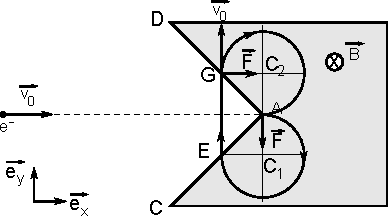
\includegraphics[width=.5\linewidth]{miroir_mag-corr}
            \captionof{figure}{Trajectoire dans la zone.}
            \label{fig:miroir_mag_corr}
        \end{center}

    \item La particule ressort par la face AC en E, avec une vitesse selon
        $\ey$ car le triangle AC$_1$E est isocèle et rectangle en C$_1$. 

    \item En dehors de la zone grisée, la particule est isolée, donc elle est
        animée d'un mouvement rectiligne uniforme ($\vf=v_0\ey=\vcte$) dans le
        référentiel du laboratoire supposé galiléen. \bigbreak

        La particule entre à nouveau dans le zone où règne le champ magnétique
        par la face AD, avec une vitesse $\vf=v_0\ey$. La trajectoire est
        alors circulaire de même rayon $R$ (car la vitesse est la même en
        norme). On représente la force magnétique en G, et on en déduit le
        position C$_2$ du centre de la trajectoire. La particule arrive en A
        avec la vitesse $\vf=-v_0\ex$ et sort de la zone grisée. \bigbreak
	
        Au final, la particule a subi une déviation de $\pi$, comme si elle
        avait été réfléchie par un miroir. On pourrait donc appeler ce
        dispositif un \textbf{miroir magnétique}.
	
        \begin{rexem}{Remarque}
            Vérifiez que l'effet miroir est maintenu si la particule incidente
            n'arrive plus en A. On constate en revanche que la particule
            n'emprunte plus le même chemin qu'à l'aller. 
        \end{rexem}
\end{enumerate}

\section{Imprimante jet d'encre}
\begin{enumerate}
    \item La gouttelette est chargée positivement, et subit la force électrique
        $\Ff_e = q\Ef$. Pour aller dans le sens des $y$ croissants, il faut que
        $\Ef$ soit selon $\uy$, comme indiqué dans l'énoncé. Or, $\Ef = -\gd V$,
        donc $\Ef$ va des \textbf{hauts potentiels} vers les \textbf{bas
        potentiels}~; il faut donc $V_1 > V_2$, soit
        \[\boxed{V_1 - V_2 > 0}\]
    \item La gouttelette a un volume $V$ et une masse volumique $\rho$. On en
        déduit
        \begin{gather*}
            \boxed{m = \rho V}
            \qavec
            \left\{
                \begin{array}{rcl}
                    \rho & = & \SI{1.0e3}{kg.m^{-3}}\\
                    V & = & \SI{10}{pL} = \SI{10e-12}{(dm)^3}\\
                      & = & \SI{1.0e-11}{(10^{-1}m)^3}\\
                      & = & \SI{1.0e-14}{m^3}
                \end{array}
            \right.\\\AN
            \boxed{m = \SI{1.0e-11}{kg}}
        \end{gather*}
        Ainsi, on trouve
        \[
            \norm{\Ff_e} = qE \approx \SI{1.7e-8}{N}
            \qet
            \norm{\Pf} = mg \approx \SI{1.0e-10}{N}
            \qsoit
            \boxed{\norm{\Ff_e} \approx 200\times\norm{\Pf}}
        \]
        On peut donc négliger le poids devant la force de \textsc{Lorentz}.
    \item On applique le PFD à la gouttelette dans le référentiel de la salle
        d'impression, supposé galiléen, avec un repère cartésien tel qu'indiqué
        sur le schéma~:
        \begin{gather*}
            m\af = q\Ef
            \Ra
            \left\{
                \begin{aligned}
                    m\xpp &= 0\\
                    m\ypp &= 0\\
                    m\zpp &= qE
                \end{aligned}
            \right.
            \Ra
            \left\{
                \begin{aligned}
                    \xp &= v_0\\
                    \yp &= \frac{qE}{m}t
                \end{aligned}
            \right.
            \Ra
            \left\{
                \begin{aligned}
                    x(t) &= v_0t\\
                    y(t) &= \frac{qE}{2m}t^2
                \end{aligned}
            \right.
        \end{gather*}
        en intégrant une première fois avec $\xp(0) = v_0$ et $\yp(0) = 0$, en
        ignorant le mouvement en $z$, puis en intégrant une seconde fois, avec
        $x(0) = 0 = y(0)$.  On trouve alors l'équation de la trajectoire~:
        \[\boxed{y(x) = \frac{qE}{2mv_0{}^2}x^2}\]
        qui est l'équation d'une parabole. Ainsi, on trouve $Y_1 = y(L_1)$~:
        \[\boxed{Y_1 = \SI{5.3e-3}{m} = \SI{5.3}{mm}}\]

    \item Après être sortie du déflecteur, la gouttelette n'est soumise à aucune
        action sauf son poids, que l'on ignore sur la durée du trajet restant
        ($v_0 = \SI{20}{m.s^{-1}}$)~: sa trajectoire est donc rectiligne et
        uniforme.

    \item On trouve l'angle de sortie en prenant
        \[\tan\tt = \dv{y}{x} = \frac{\yp(L_1)}{\xp(L_1)} =
        \frac{qEL_1}{mv_0{}^2} = 2\frac{Y_1}{L_1}\]
        L'angle trouvé étant petit ($\tt \approx \SI{0.21}{rad}$), $\tan\tt
        \approx \tt \approx \sin\tt$. Or, on a
        \begin{gather*}
            Y_2 = Y_1 + L_2\sin\tt
            \\\Ra
            \boxed{Y_2 = Y_1\left(1+2\frac{L_2}{L_1}\right)}
            \qavec
            \left\{
                \begin{array}{rcl}
                    Y_1 & = & \SI{5.3e-1}{cm}\\
                    L_1 & = & \SI{5.0}{cm}\\
                    L_2 & = & \SI{20}{cm}
                \end{array}
            \right.\\\AN
            \boxed{Y_2 = \SI{4.8}{cm}}
        \end{gather*}
\end{enumerate}
\end{document}
